\chapter{Introduction}

\section{Overview of neutron halo nuclei}
Over recent years, the study of neutron-rich nuclei has increasing attention in the field of nuclear physics, providing invaluable insights into the conventional nuclear models and interactions in the environment far from stable nuclei. One particularly intriguing subclass is neutron halo nuclei\cite{Tanihata96}, which feature an extended halo of one or two loosely bound neutrons far from its core. The first discovery of neutron halo nucleus was ${}^{11}$Li by I. Tanihata et al\cite{Tanihata85}. 
%In Figure \ref{fig:Radius_11Li},
In figure 1.1, ${}^{11}$Li has enormously large radius compared to neighboring  He, Li, Be and C isotopes which has similar A number. Based on this discovery, he suggested that ${}^{11}$Li has a large deformation or a long tail in matter distribution. After that, P. G. Hansen and B. Jonson\cite{HansenandJonson} suggested ${}^{11}$Li as a neutron halo nuclei due to the large neutron radius compared to its core ${}^{9}$Li.

\begin{figure}
    \centering
    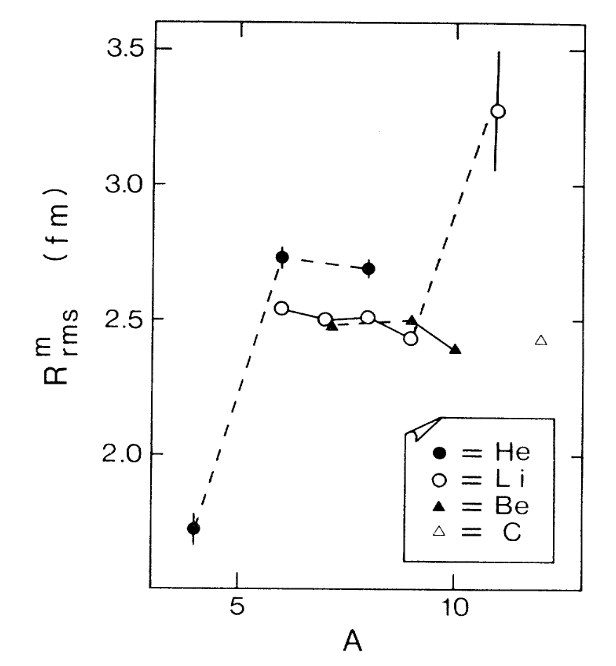
\includegraphics[width=6cm]{chapter1/Radius_of_11Li.png}
    \caption[Matter rms radius of He, Li, Be and C isotopes.]{Matter rms radius of He, Li, Be and C isotopes. ${}^{11}$Li has significantly large radius compared to neighboring He, Li, Be, and C isotopes. \cite{Tanihata85}}
    \label{fig:Radius_11Li}
\end{figure}

After more research on neutron halo nucleus, many research suggested how to decide a nuclei as a halo nuclei. One is obviously a small neutron separation energy. Compared to the separation energy of stable nuclei around 6 - 8 MeV, neutron halo nuclei have extremely small separation energy less than 1 MeV. And because of this, neutron halo nuclei have large radius. We can see this relationship between neutron separation energy and large radius from simple assumption  Given that the neutron wavefunction is a square well potential, the wavefunction of neutron can be written,
\begin{align}
    \Psi(r) = \bigg(\frac{2\pi}{k}\bigg)\bigg(\frac{-e^{k r}}{r}\bigg)\bigg[\frac{e^{k R}}{(1+ k R)^{1/2}}\bigg], \label{eq:wavefunction}
\end{align}
where R is the width of the potential. With wavefunction, the density distribution of the neutron is
\begin{align}
    \rho(r) = |\Psi(r)|^2 \propto \frac{e^{-2k r}}{r^2}.
\end{align}
The factor $k$ determines the tail of the neutron, and it is related to the neutron separation energy as
\begin{align}
    (\hbar k)^2 = 2\mu S_n,
\end{align}
where $\mu$ is the effective mass of system and $S_n$ is the neutron separation energy. From this equation, we can see that the $k$ is inversely proportional to the neutron separation energy. The smaller the neutron separation energy is, the larger the $k$ is. And the larger the $k$ is, the longer tail of neutron is. So, the halo nuclei usually have small neutron separation energy and large radius.

% halo feature 2
The narrow momentum distribution is also the feature of halo nuclei. The momentum distribution of neutron [$f (p)$] can be expressed by the Fourier transform of the wavefunction \ref{eq:wavefunction},
\begin{align}
    f(p) = \frac{C}{p^2+(\hbar k)^2},
\end{align}
where $p$ is the momentum of the neutron and the width of the distribution is defined by $k$ which related with separation energy. Here, you can see the concept of Heisenberg uncertainty principle. The smaller the $k$, the wider the density distribution, and the narrower the momentum distribution. 

\begin{figure}
    \centering
    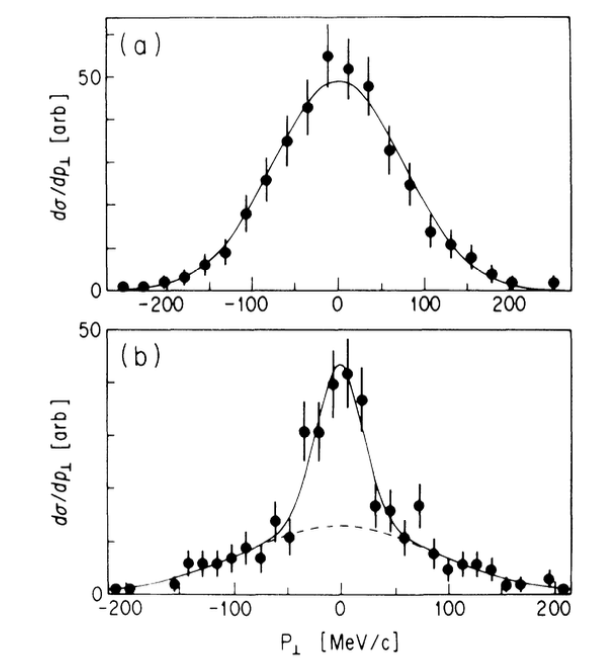
\includegraphics[width=7cm]{chapter1/Momentum_distribution.png}
    \caption[The momentum distribution of ${}^{6}$H and ${}^{9}$Li]{The momentum distribution of (a) ${}^{6}$H from ${}^{8}$H + C reaction, and (b) ${}^{9}$Li from ${}^{11}$Li + C reaction. ${}^{9}$Li has extremely narrow momentum distribution, where the narrow Gaussian peak has $\sigma  = 23 \pm 5$ MeV/c. \cite{Kobayashi88}}
    \label{fig:Momentum_distribution}
\end{figure}

In figure \ref{fig:Momentum_distribution}, the momentum distribution of ${}^{6}$H and ${}^{9}$Li are shown. ${}^{6}$H has a large width of momentum distribution, $\sigma = 77 \pm 5$ MeV/c, because of the non halo structure of ${}^{8}$H. On the other hand, ${}^{9}$Li has a very narrow momentum distribution where the Gaussian peak has $\sigma  = 23 \pm 5$ MeV/c. This narrow momentum distribution can be interpreted ${}^{11}$Li as a halo nucleus.

% halo feature 3
Another key parameter defining the configuration of halo nuclei is the orbital angular momentum of the valence neutron. The momentum distribution's shape is influenced not only by the separation energy but also by the orbital's angular momentum ($l$) due to the centrifugal barrier. The barrier's width is proportional to $l(l+1)/r^2$, which significantly impacts the neutron's density distribution. Riisager et al. \cite{Riisager} have performed calculations on the radius of a one-neutron halo system in a square-well potential for varying separation energies and orbital angular momenta. In Figure \ref{fig:Angular_Orbital}, the x-axis represents the separation energy normalized by the size of the well potential $R_0$, while the y-axis shows the root-mean-square (rms) radius, also normalized by $R_0$.  It is observed that the rms radius for $l$ = 0 or $l$ = 1 tends to increase significantly as the separation energy approaches zero, indicative of halo formation. However, for $l$ = 2, the rms radius remains close to $R_0$, indicating that it is challenging for nuclei with $l$ = 2 or higher to develop a halo structure.

\begin{figure}
    \centering
    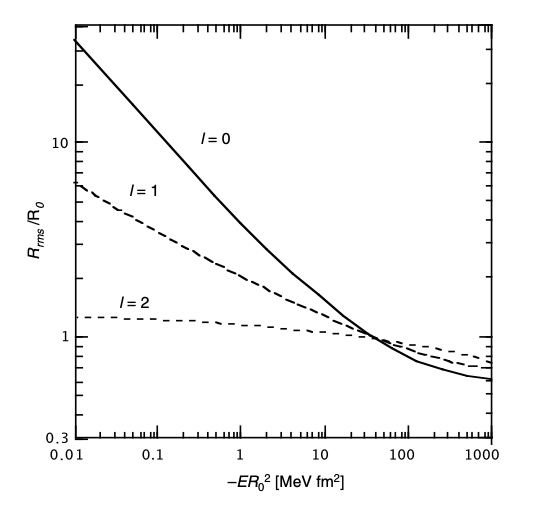
\includegraphics[width=8cm]{chapter1/Angular_Orbital.png}
    \caption{RMS radius of one neutron halo for different separation energies and orbitals. \cite{Riisager}}
    \label{fig:Angular_Orbital}
\end{figure}

%Also in three-body halo system, the centrifugal barrier is defined in the form of $[(K+3/2)(K+5/2)]/\rho^2$ by D. V. Fedorov et al.\cite{Fedorov} with the quantum number $K$ (usually called hypermomenent). In this formula, the hight of centrifugal barrier rapidly increases with $K$. Ad even $K = 0$ has centrifugal barrier.
Through the consideration about halo nuclei so far, we can understand the mechanism of development of halo structure. The halo structure can be developed when the neutron separation energy is small and the orbital angular momentum is low. With small neutron separation energy and low angular momentum, the 

% halo feature 4
The most important feature of a halo nucleus focused on this research is soft mode of electric dipole excitation. Given that halo nuclei has a core and loosely bounded valance neutron, the core and valance neutron can be polarized by the external electric field. And this dipole excitation mode is shown in very low energy region, because the halo structure response easily to the external electric field. Compared to Giant dipole moment (GDR) which is the dipole excitation mode of stable nuclei, the soft dipole mode is shown in very low energy region. In figure \ref{fig:E1_response}, the schematic representation of the giant dipole resonance and soft dipole mode is shown. The giant dipole resonance is shown in high energy region, and the soft dipole mode is shown in very low energy region. The soft dipole mode is also called as pygmy dipole resonance (PDR). 
The strength of soft dipole mode can be described with E1 reduced transition probability ($B(E1)$). In E1 reduced transition probability, the term 'reduced' means that the transition matrix element is independent of the magnetic sub-state of the initial and final states from the Wigner-Eckart theorem. The E1 reduced transition probability is defined as

\begin{figure}
    \centering
    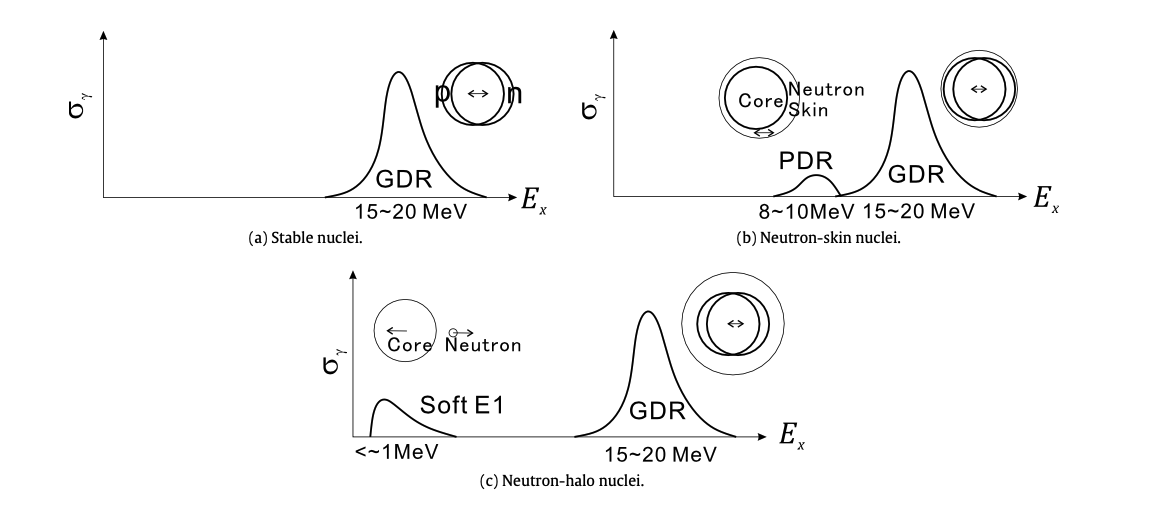
\includegraphics[width=\textwidth]{chapter1/E1_response.png}
    \caption{The schematic representation of the giant dipole resonance and soft dipole mode \cite{Nakamura17}}
    \label{fig:E1_response}
\end{figure}

This soft mode of electric dipole excitation is called Soft E1 excitation. This feature predicted by P. G. Hansen and B. Jonsen \cite{HansenandJonson}, and also K. Ikeda et al.\cite{Ikeda}. The strength of soft E1 excitation can be described with E1 reduced transition probability ($B(E1)$). In E1 reduced transition probability, the term 'reduced' means that the transition matrix element is independent of the magnetic sub-state of the initial and final states from the Wigner-Eckart theorem. The E1 reduced transition probability is defined as

\begin{align}
    B(E1) = \frac{|\langle \Phi_f ||\hat{T}(E1)|| \Phi_i\rangle|^2}{(2J_i + 1)},
\end{align}

where $\hat{T(E1)}$ is E1 transition operator, $\Phi_i$ and $\Phi_f$ are the initial and final states of the system, and $J_i$ is the total angular momentum of the initial state.
Recently, in boron isotopes, the reduced E1 transition probability of ${}^{19}$B is observed by K. J. Cook et al.\cite{KJCook} using Coulomb dissociation method. ${}^{19}$B has been considered as a two neutron halo nuclei, but on the other hand, also considered as 4 neutron halo nucleus or neutron skin nucleus. ${}^{19}$B has very small two neutron separation energy, $S_{2n} = 0.088(564)$ MeV \cite{Wang19B}, but also its core ${}^{17}$B has small 2n separation energy, $S_{2n} = 1.384(205)$ MeV and large radius\cite{Suzuki99}. And also the valance neutrons of ${}^{19}$ are occupied in sd-shell, which makes the orbital mixing of $1d_{5/2}$ and $2s_{1/2}$. If 4 neutrons occupy the $1d_{5/2}$ orbital, because of the high centrifugal barrier, halo structure cannot develope. On the other hand, if 2 neutrons occupy the $2s_{1/2}$ orbital, the halo structure can be developed. The result of K. J. Cook et al. extracted the reduced E1 transition probability of ${}^{19}$B and the peak was observed around 0.5 MeV. This result shows that the ${}^{19}$B has very strong soft E1 mode, which means that the halo structure of ${}^{19}$B is developed.

\begin{figure}[t]
    \centering
    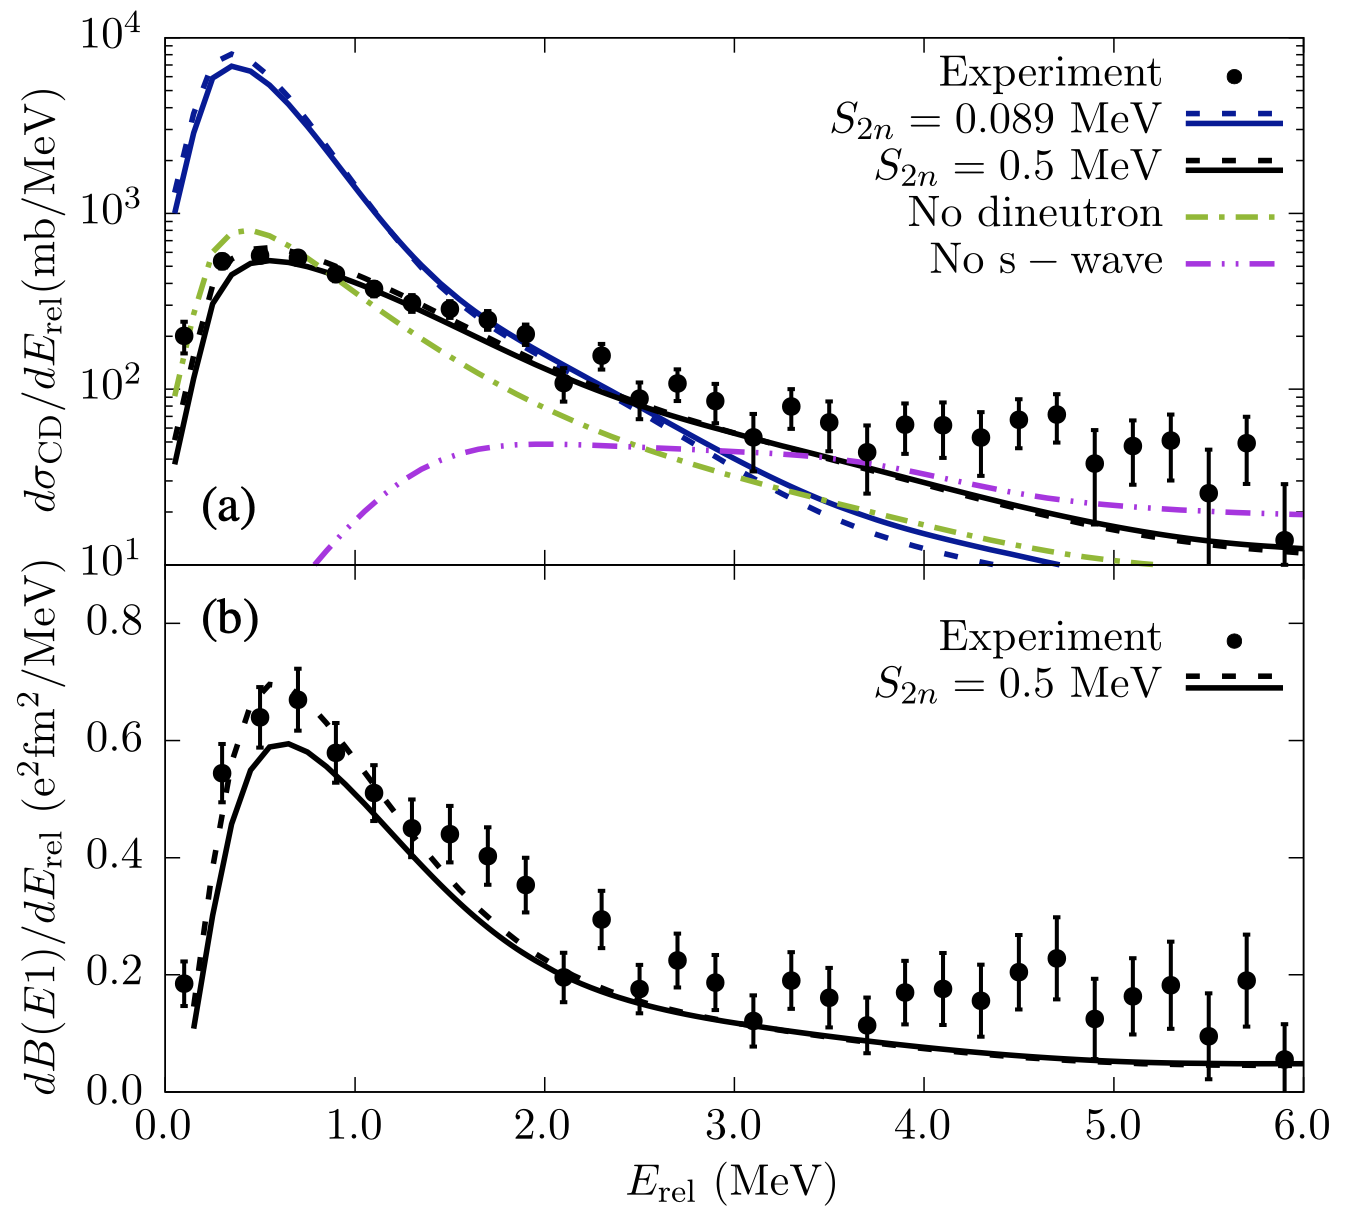
\includegraphics[width=10cm]{chapter1/19B_B(E1).png}
    \caption{The B(E1) distribution of ${}^{19}$B. The peak at 0.5 MeV is the soft E1 excitation.}
\end{figure}

\begin{figure}
    \centering
    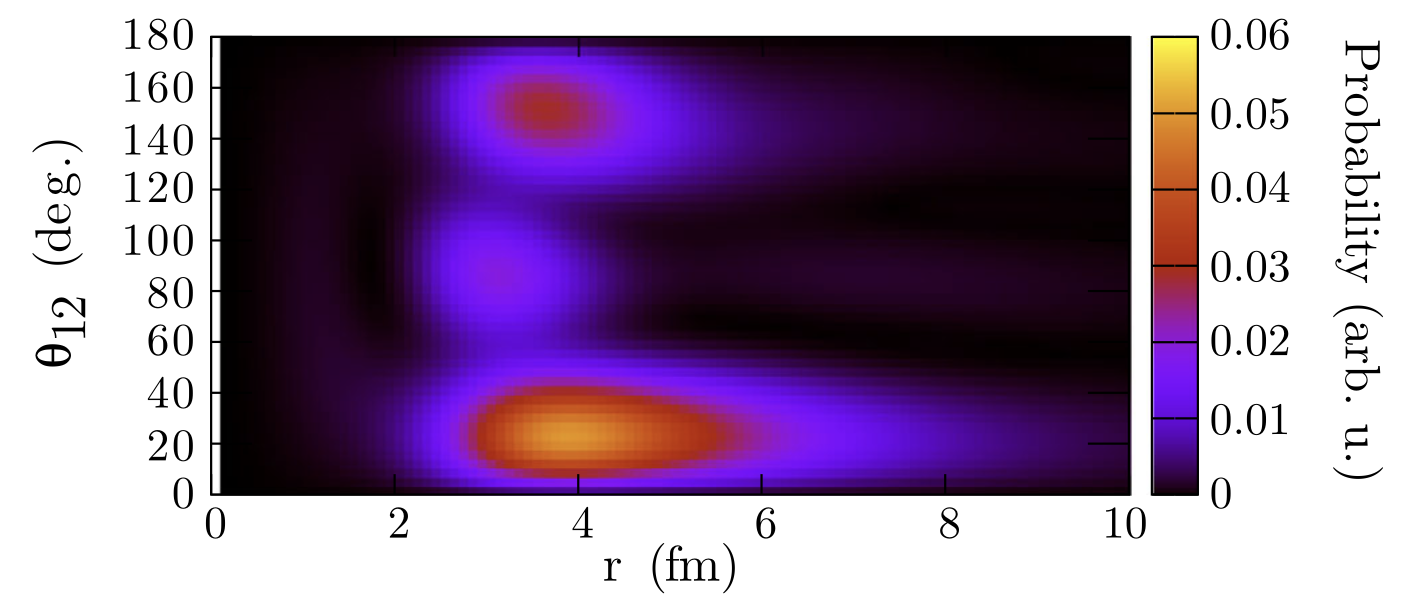
\includegraphics[width=10cm]{chapter1/19B_Dineutron.png}
    \caption{The dineutron correlation of ${}^{19}$B.}
\end{figure}

\section{The halo structure of ${}^{17}$B}

After revealing the structure of ${}^{19}$B, the structure of ${}^{17}$B got attention. The first discover of ${}^{17}$B as a halo nucleus was by T. Suzuki.\cite{Suzuki99} ${}^{17}$B has small 2n separation energy, and large radius. And also, the valance neutrons of ${}^{17}$B are occupied in sd-shell, which makes the orbital mixing of $1d_{5/2}$ and $2s_{1/2}$ as same as ${}^{19}$B. 

But recently, Z. H. Yang et al. \cite{ZHYang} shows a strong evidence that ${}^{17}$B might not be a two neutron halo nuclei. He performed the quasi-free ($p,pn$) scattering reaction and extracted the relative energy distribution of ${}^{16}$B. He assumed that the knocked-out neutron from the ${}^{17}$B  should almost come from $1d_{5/2}$ or $2s_{1/2}$ orbital and got the relative energy distribution of ${}^{16}$B. (Figure 1.3) And also, he obtained the spectroscopic factors for $1d_{5/2}$ and $2s_{1/2}$ orbital and there was surprisingly small percentage 9(2)\% of $2s_{1/2}$ orbital. This result is very different from the ones, which are 36(19)\%, 69(20)\%, 50(10)\% and by T. Suzuki and Y. Yamaguchi. \cite{Suzuki99} \cite{Suzuki} \cite{Yamaguchi} Also A. Estradé et al. \cite{Estrade} shows proton radii of boron isotope. In this research, ${}^{17}$B has very thick neuron surface, 0.51(11) fm, which indicates a ${}^{15}$B core modification. 

\begin{figure}
    \centering
    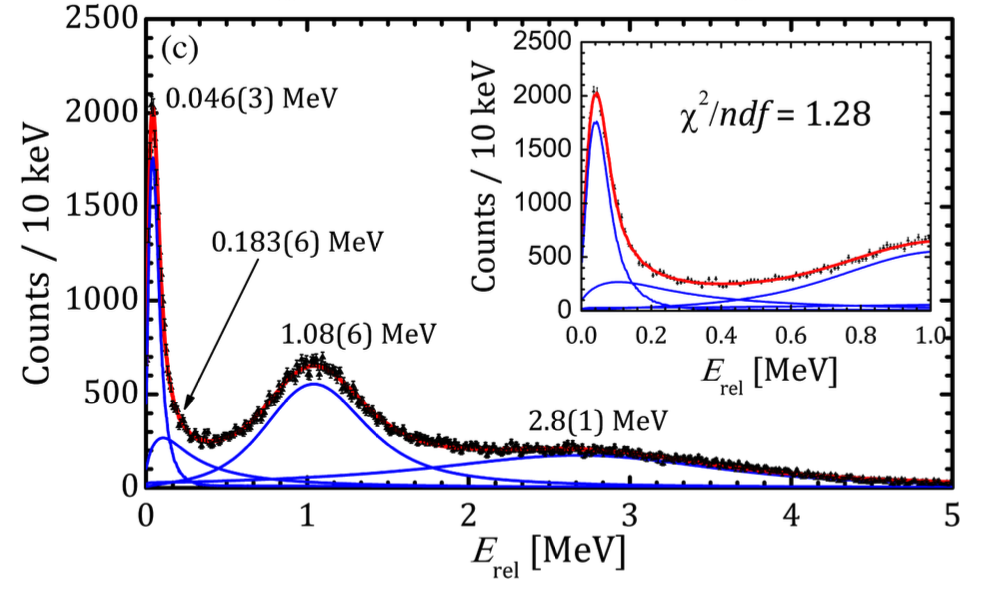
\includegraphics[width=10cm]{chapter1/17B_ZHYang.png}
    \caption{The relative energy distribution of ${}^{16}$B.\cite{ZHYang}}
\end{figure}

\begin{figure}
    \centering
    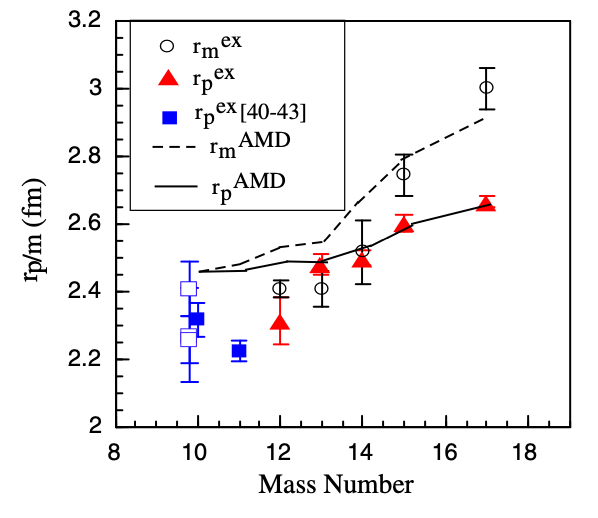
\includegraphics[width=8cm]{chapter1/RadiiofBoron.png}
    \caption{The proton radii ($r_p$) and rms matter radii ($r_m$) of ${}^{12-17}$B. \cite{Estrade}}
\end{figure}
So, in this research, we study the Soft E1 excitation of ${}^{17}$B for the first, which can be the final key for deciding ${}^{17}$B as a halo nuclei or not. In this thesis, we will discuss the Coulomb Dissociation of ${}^{17}$B as a tool for searching the Soft E1 excitation of ${}^{17}$B. 

%\begin{align}
    %\Psi({}^{17}\text{B}) = \psi({}^{15}\text{B}) \otimes [\alpha |1d_{5/2} \rangle^2 + \beta |2s_{1/2} \rangle^2]
%\end{align}

